\chapter{Výsledky}\label{cha:vysledky}

V této kapitole shrnujeme výsledky vybraných architektur z kapitoly \nameref{cha:experimenty} na testovacích datech a provádíme kvantitativní a kvalitativní srovnání se state-of-the-art systémy pro extrakci melodie, představené v kapitole \nameref{cha:souvisejici}.

\section{Výběr testovaných modelů}

Pro srovnání jsme vybrali nejlepší natrénované modely z kapitoly \nameref{cha:experimenty} od každé testované architektury. Každou vybranou architekturu krátce popíšeme a v tabulce uvedeme nalezené nastavení hyperparametrů.

Všechny testované modely mají společnou reprezentaci cílového výstupu při trénování. Rozlišení diskretizace výšky noty je nastaveno na 5 hodnot na půltón, rozptyl distribuce výšky noty je nastaven na 0.18, na základě experimentů v sekci \nameref{sec:crepe}.

Modely byly trénovány pomocí grafické karty NVIDIA GeForce GTX 1070.

\subsection{Architektura CREPE}

Zvolený model dosáhl na validačních datech přesnosti odhadu výšky 0.682 a přesnosti odhadu výšky nezávisle na oktávě 0.783. Počet trénovatelných parametrů tohoto modelu je $2\,016\,350$. Proběhlo $360\,000$ iterací trénování. Trénování probíhalo přes dvě hodiny. Parametry vybrané architektury uvádíme v tabulce \ref{tab:crepe_hyperparams}.

\begin{table}[p]
\centering
\begin{tabular}{llll}
\toprule
Prohledávané parametry               &          & Ostatní parametry &         \\
Parametr                             & Hodnota  & Parametr          & Hodnota \\
\midrule
Multiplikační koef. kapacity         & 8        & Velikost dávky    & 32      \\
Šířka vstupního okna                 & 2048     & Iterace trénování & 360000         \\
Násobné rozlišení první vrstvy       & 6 vrstev & Learning rate     & 0.001   \\
\bottomrule
\end{tabular}
\caption{Nastavení architektury a hyperparametrů pro testovanou architekturu CREPE.}\label{tab:crepe_hyperparams}
\end{table}


\subsection{Architektura WaveNet}

Zvolený model dosáhl na validačních datech přesnosti odhadu výšky 0.673 a přesnosti odhadu výšky nezávisle na oktávě 0.768. Počet trénovatelných parametrů tohoto modelu je $5\,206\,524$. Proběhlo $360\,000$ iterací trénování. Trénování probíhalo téměř pět hodin. Parametry vybrané architektury uvádíme v tabulce \ref{tab:wavenet_hyperparams}.

\begin{table}[p]
\centering
\begin{tabular}{llll}
\toprule
Prohledávané parametry               &          & Ostatní parametry &         \\
Parametr                             & Hodnota  & Parametr          & Hodnota \\
\midrule
Velikost první konvoluce & 0      & Iterace trénování     & 100000 \\
Počet filtrů  & 16     & Velikost dávky    & 8      \\
Počet bloků            & 2     & Learning rate & 0.001       \\
Maximální dilatace         & 1024   &                &        \\
Transformace skip propojení & concat &                &        \\
\bottomrule
\end{tabular}
\caption{Nastavení architektury a hyperparametrů pro testovanou architekturu WaveNet.}\label{tab:wavenet_hyperparams}
\end{table}

\subsection{Architektura HCNN}

Pro úspěšnost modelů na validačních datech jsme se rozhodli porovnat dvě různé architektury HCNN. Architekturu s minimálním kontextem $5.8\,\rm ms$, dále nazývanou HCNN noctx, a architekturu, která uvažuje širší kontext, dále jen HCNN.

\subsubsection{HCNN noctx}

Zvolený model dosáhl na validačních datech přesnosti odhadu výšky 0.751 a přesnosti odhadu výšky nezávisle na oktávě 0.813. Počet trénovatelných parametrů tohoto modelu je $27\,857$. Proběhlo $100\,000$ iterací trénování. Trénování probíhalo 22 minut. Parametry vybrané architektury uvádíme v tabulce \ref{tab:hcnnnoctx_hyperparams}.

\begin{table}[p]
\centering
\begin{tabular}{llll}
\toprule
Prohledávané parametry               &          & Ostatní parametry &         \\
Parametr                             & Hodnota  & Parametr          & Hodnota \\
\midrule
Parametr \texttt{hop\_size} & 256       & Iterace trénování                       & 100000 \\
Kontext                & noctx         & Velikost dávky                      & 16     \\
Vstupní reprezentace   & HCQT       & Learning rate                   & 0.001  \\
Filtry, Bloky                 & 16, 8        & Dropout                          & 0.3    \\
Harmonická trans. & $\pm 12$, $\pm 19$ &  &       \\
\bottomrule
\end{tabular}
\caption{Nastavení architektury a hyperparametrů pro testovanou architekturu HCNN noctx.}\label{tab:hcnnnoctx_hyperparams}
\end{table}
\begin{table}[p]
\centering
\begin{tabular}{p{4.5cm}p{3cm}ll}
\toprule
Prohledávané parametry               &          & Ostatní parametry &         \\
Parametr                             & Hodnota  & Parametr          & Hodnota \\
\midrule
Parametr \texttt{hop\_size} & 256     & Iterace trénování                       & 100000 \\
Kontext            & 3\_last\_layers \_wavenet & Velikost dávky                      & 8      \\
Vstupní reprezentace    & Vícekan. HCQT & Learning rate                   & 0.001  \\
Filtry, Bloky & 16, 4      & Dropout                          & 0.3    \\
Harmonická trans. & $\pm 12$&   &       \\
Pst. augmentace       & 0.75    &                                  &        \\
\bottomrule
\end{tabular}
\caption{Nastavení architektury a hyperparametrů pro testovanou architekturu HCNN.}\label{tab:hcnn_hyperparams}
\end{table}

\subsubsection{HCNN}

Zvolený model dosáhl na validačních datech přesnosti odhadu výšky 0.755 a přesnosti odhadu výšky nezávisle na oktávě 0.828. Počet trénovatelných parametrů tohoto modelu je $23\,153$. Proběhlo $100\,000$ iterací trénování. Trénování probíhalo 75 minut. Parametry vybrané architektury uvádíme v tabulce \ref{tab:hcnn_hyperparams}.

\subsection{Detekce melodie}

Pro detekci melodie z vypočítané funkce salience jsme použili techniku práhování (thresholding). Pro odhad přítomnosti melodie nalezneme maximální hodnotu funkce salience v daném okamžiku --- pokud tato hodnota přesahuje jistý práh, daný časový okamžik se uvažuje jako obsahující melodii. Konkrétní nastavení práhu jsme určili na základě validačních dat pro každou metodu zvlášť. Tato metoda práhování je použita například také v práci \cite{Bittner2017}.

\section{Kvantitativní srovnání}

% , která je představuje evaluační páteř oboru a je každoročně pořádána pro nezávislé srovnávání metod úloh Music Information Retrieval

V tabulkách \ref{tab:vysledky_OA}, \ref{tab:vysledky_RPA}, \ref{tab:vysledky_RCA}, \ref{tab:vysledky_VR} a \ref{tab:vysledky_VFA} prezentujeme výsledky nově představovaných metod v porovnání s velmi silnými baseline metodami pro extrakci melodie. Jak uvádíme v kapitole \nameref{cha:souvisejici}, práce \cite{Salamon2012a} dosahuje spolu s prací \cite{Dressler2009} v průměru nejlepších výsledků v soutěži MIREX. Práce \cite{Bittner2017} a \cite{DBasaranSEssid2018} představují metody, které dosahují nejlepších výsledků na prozatím nejrozmanitějším datasetu MedleyDB. 

Pro srovnání metod používáme datasety ADC04, MIREX05train a ORCHSET, které jsme v práci vyhradili pouze pro testování. Také používáme testovací množiny datasetů MedleyDB a MDB-melody-synth, převzaté z prací \cite{Bittner2017} a \cite{DBasaranSEssid2018}, pro dataset WJazzD používáme vlastní testovací množinu. Metodika výběru příkladů do testovací množiny WJazzD je popsána v kapitole \nameref{cha:datasety}, všechny množiny jsou výčtem popsány v elektronické příloze.

V následujících tabulkách uvádíme standardní metriky, používané pro srovnání metod pro extrakci melodie, jde o metriky celkové přesnosti (OA), přesnosti odhadu výšky (RPA), přesnosti odhadu výšky nezávisle na oktávě (RCA), úplnosti detekce melodie (VR) a nesprávné detekce (VFA). Připomínáme, že metrika celkové přesnosti (OA) zahrnuje vyhodnocení odhadu výšky i vyhodnocení detekce melodie, zbylé metriky měří úspěšnost pouze jedné z obou podúloh. K vyhodnocování používáme knihovnu \texttt{mir\_eval}, která poskytuje transparentní a standardizovaný způsob výpočtu metrik pro úlohy oboru Music Information Retrieval.

\begin{table}[p]
\centering
\scalebox{1.0}{%
\begin{tabular}{lrrrrrr}
\toprule
Metoda & ADC04 & \shortstack[r]{MDB-m-s\\ test} & \shortstack[r]{MIREX05\\train.} & \shortstack[r]{MDB\\test} & \shortstack[r]{ORCH-\\SET} & \shortstack[r]{WJazzD\\test} \\
\midrule
    Salamon &         0.714 &           0.527 &          0.715 &         0.519 &        0.235 &        0.667 \\
    Bittner &         0.716 &           0.633 &          0.702 &         0.611 &        0.407 &        0.692 \\
    Basaran &         0.669 &   \textbf{0.689}&          0.734 &         0.640 &\textbf{0.483}&        0.700 \\
\arrayrulecolor{black!30}\midrule
      CREPE &         0.590 &           0.562 &          0.652 &         0.502 &        0.248 &        0.671 \\
    WaveNet &         0.681 &           0.528 &          0.649 &         0.503 &        0.256 &        0.648 \\
 HCNN noctx & \textbf{0.737}&           0.626 &          0.723 &         0.635 &        0.439 &        0.715 \\
       HCNN &         0.726 &           0.661 &  \textbf{0.755}& \textbf{0.652}&        0.459 &\textbf{0.725} \\
\arrayrulecolor{black}\bottomrule
\end{tabular}
}%
\caption{Výsledky celkové přesnosti (Overall Accuracy). Vyznačené výsledky jsou pro daný dataset nejvyšší z porovnávaných v rámci daného datasetu.}\label{tab:vysledky_OA}
\end{table}

\begin{table}[p]
\centering
\scalebox{1.0}{%
\begin{tabular}{lrrrrrr}
\toprule
Metoda & ADC04 & \shortstack[r]{MDB-m-s\\ test} & \shortstack[r]{MIREX05\\train.} & \shortstack[r]{MDB\\test} & \shortstack[r]{ORCH-\\SET} & \shortstack[r]{WJazzD\\test} \\
\midrule
    Salamon &          0.767 &           0.514 &          0.761 &         0.526 &         0.281 &        0.693 \\
    Bittner &          0.814 &           0.606 &          0.807 &         0.670 &         0.519 &        0.774 \\
    Basaran &          0.793 &   \textbf{0.733}&          0.798 &         0.706 & \textbf{0.635}&        0.767 \\
\arrayrulecolor{black!30}\midrule
      CREPE &          0.794 &           0.550 &          0.779 &         0.616 &         0.408 &        0.782 \\
    WaveNet &          0.796 &           0.528 &          0.792 &         0.595 &         0.345 &        0.759 \\
 HCNN noctx &          0.827 &           0.647 &          0.833 &         0.701 &         0.511 &        0.805 \\
       HCNN &  \textbf{0.841}&           0.654 &  \textbf{0.851}& \textbf{0.715}&         0.535 &\textbf{0.806}\\
\arrayrulecolor{black}\bottomrule
\end{tabular}
}%
\caption{Výsledky přesnosti odhadu výšky (Raw Pitch Accuracy). Vyznačené výsledky jsou pro daný dataset nejvyšší z porovnávaných v rámci daného datasetu.}\label{tab:vysledky_RPA}
\end{table}

\begin{table}[p]
\centering
\scalebox{1.0}{%
\begin{tabular}{lrrrrrr}
\toprule
Metoda & ADC04 & \shortstack[r]{MDB-m-s\\ test} & \shortstack[r]{MIREX05\\train.} & \shortstack[r]{MDB\\test} & \shortstack[r]{ORCH-\\SET} & \shortstack[r]{WJazzD\\test} \\
\midrule
    Salamon &        0.807 &        0.639 &        0.805 &         0.659 &         0.568 &             0.757 \\
    Bittner &        0.855 &        0.666 &        0.824 &         0.735 &         0.694 &             0.785 \\
    Basaran &        0.820 &\textbf{0.766}&        0.807 &         0.757 & \textbf{0.776}&             0.776 \\
\arrayrulecolor{black!30}\midrule
      CREPE &        0.851 &        0.617 &        0.810 &         0.714 &         0.607 &             0.808 \\
    WaveNet &        0.843 &        0.597 &        0.828 &         0.703 &         0.564 &             0.793 \\
 HCNN noctx &        0.862 &        0.699 &        0.845 &         0.767 &         0.683 &     \textbf{0.821}\\
       HCNN &\textbf{0.880}&        0.716 &\textbf{0.863}& \textbf{0.781}&         0.732 &             0.820 \\
\arrayrulecolor{black}\bottomrule
\end{tabular}
}%
\caption{Výsledky přesnosti odhadu výšky nezávisle na oktávě (Raw Chroma Accuracy). Vyznačené výsledky jsou pro daný dataset nejvyšší z porovnávaných v rámci daného datasetu.}\label{tab:vysledky_RCA}
\end{table}


\begin{table}[h]
\centering
\scalebox{1.0}{%
\begin{tabular}{lrrrrrr}
\toprule
Metoda & ADC04 & \shortstack[r]{MDB-m-s\\ test} & \shortstack[r]{MIREX05\\train.} & \shortstack[r]{MDB\\test} & \shortstack[r]{ORCH-\\SET} & \shortstack[r]{WJazzD\\test} \\
\midrule
\arrayrulecolor{black!30}\midrule
    Salamon &          0.774 &       \bf{0.729}&      \bf{0.841}&         0.705 &       0.603 &       0.794 \\
    Bittner &          0.796 &           0.638 &          0.796 &         0.675 &       0.614 &       0.846 \\
    Basaran &          0.732 &           0.704 &          0.713 &         0.676 &       0.605 &       0.841 \\
      CREPE &          0.584 &           0.431 &          0.576 &         0.449 &       0.326 &       0.680 \\
    WaveNet &          0.765 &           0.595 &          0.747 &         0.618 &       0.494 &       0.784 \\
 HCNN noctx &      \bf{0.806}&           0.684 &          0.824 &         0.728 &   \bf{0.729}&   \bf{0.880}\\
       HCNN &          0.794 &           0.692 &          0.836 &     \bf{0.741}&       0.721 &       0.872 \\
\arrayrulecolor{black}\bottomrule
\end{tabular}
}%
\caption{Výsledky úplnosti detekce (Voicing Recall).}\label{tab:vysledky_VR}
\end{table}
\begin{table}[h]
\centering
\scalebox{1.0}{%
\begin{tabular}{lrrrrrr}
\toprule
Metoda & ADC04 & \shortstack[r]{MDB-m-s\\ test} & \shortstack[r]{MIREX05\\train.} & \shortstack[r]{MDB\\test} & \shortstack[r]{ORCH-\\SET} & \shortstack[r]{WJazzD\\test} \\
\midrule
\arrayrulecolor{black!30}\midrule
    Salamon &      \bf{0.103}&           0.394 &          0.263 &         0.300 &        0.385 &       0.271 \\
    Bittner &          0.278 &           0.273 &          0.308 &         0.306 &        0.490 &       0.333 \\
    Basaran &          0.188 &           0.271 &      \bf{0.160}&         0.290 &        0.407 &       0.274 \\
      CREPE &          0.178 &       \bf{0.252}&          0.171 &     \bf{0.243}&    \bf{0.235}&   \bf{0.213}\\
    WaveNet &          0.311 &           0.383 &          0.387 &         0.397 &        0.426 &       0.370 \\
 HCNN noctx &          0.246 &           0.312 &          0.336 &         0.333 &        0.535 &       0.339 \\
       HCNN &          0.222 &           0.258 &          0.278 &         0.310 &        0.511 &       0.300 \\
\arrayrulecolor{black}\bottomrule
\end{tabular}
}%
\caption{Výsledky nesprávné detekce (Voicing False Alarm). Nižší hodnota je lepší.}\label{tab:vysledky_VFA}
\end{table}


\subsection{Popis výsledků}

Metody HCNN a HCNN noctx překonávají srovnávané algoritmy v metrikách celkové přesnosti (OA), přesnosti odhadu výšky (RPA) a přesnosti odhadu výšky nezávisle na oktávě (RCA) na datasetech ADC04, MIREX05train a WJazzD. Metoda HCNN pak překonává všechny srovnávané přístupy i na datasetu MedleyDB. Na obrázku \ref{obr:final_medleydb} porovnáváme rozdělení dosažených výsledků na datasetu MedleyDB, na uvedeném krabicovém grafu lze navíc porovnat rozptyl výsledků. V metrice RCA metody HCNN dosahují menší variability na sadě testovacích příkladů. Na zbylých datasetech MDB-melody-synth a ORCHSET překonává architektura HCNN ve všech uvažovaných metrikách pouze práce \cite{Salamon2012a} a \cite{Bittner2017}.

Co se týče zbylých architektur CREPE a WaveNet, v metrikách přesnosti odhadu výšky (RPA) a přesnosti odhadu výšky nezávisle na oktávě (RCA) na téměř všech testovacích datasetech překonávají metodu \cite{Salamon2012a}, která není založena na strojovém učení. Výsledky v porovnání s HCNN, \cite{Bittner2017} a \cite{DBasaranSEssid2018} jsou však až na výjimky nižší.

Podle očekávání na základě výsledků ze soutěže MIREX se na datasetu ORCHSET výsledky algoritmů liší nejvíce, v některých případech až o desítky procent. Jak popisujeme v kapitole \nameref{cha:datasety}, dataset je složen z orchestrálních nahrávek a kvůli vysokému stupni polyfonie a rozmanitým kombinacím barev nástrojů se jedná pro metody extrakce melodie o velmi náročný materiál. Naopak nejblíže, zejména v metrikách RPA a RCA, jsou si výsledky na datasetech ADC04, MIREX05train a WJazzD. Výňatky v těchto datasetech často obsahují velmi zřetelnou melodii a v porovnání s datasetem MedleyDB je jejich hudební obsah žánrově homogenní.

Vzhledem k dosaženým výsledkům, jednoduchosti sítí a rychlému trénování považujeme návrh architektury HCNN jako nadějný podklad pro navazující práci. Abychom mohli uvedené výsledky interpretovat, provedeme nejprve také kvalitativní srovnání algoritmů. 

% \textcolor{red}{dopsat}
% - basaran má vyhlazování, bittnerová ne, tu překovávám vždy (porovnat velikosti oken)

\begin{figure}[h]\centering
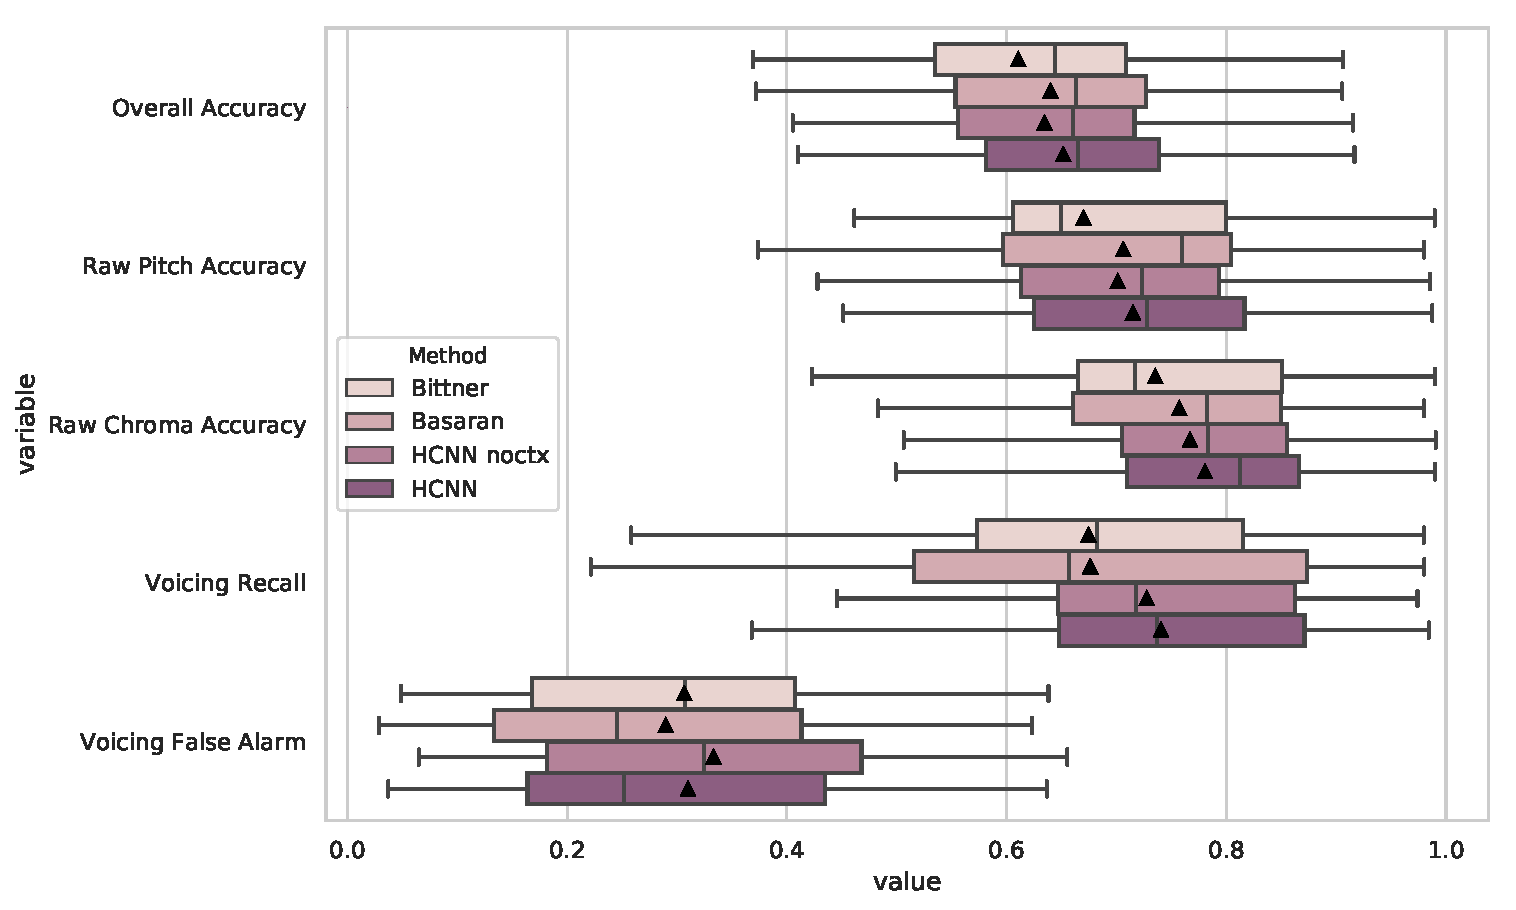
\includegraphics[width=\textwidth,height=\textheight,keepaspectratio]{../img/final_medleydb}
\caption{Výsledky nejúspěšnějších metod na datasetu MedleyDB}
\label{obr:final_medleydb}
\end{figure}

\section{Kvalitativní srovnání}

Na základě kvantitativního vyhodnocení vybíráme metody Bittnerové a Basarana pro podrobnější srovnání na jednotlivých příkladech. Z testovaných architektur pak vybíráme obě varianty HCNN. V následujících srovnáních se soustředíme na odhad výšky, proto v obrázcích zobrazujeme pouze části odhadů, ve kterých podle referenční anotace melodie zní. Obrázky jsou bez tohoto zjednodušení příliš komplikované a v práci detekci melodie řešíme pouze okrajově. Metodika výběru kvalitativních příkladů spočívala v hledání skladeb, ve kterých se odhady jednotlivých algoritmů vzájemně nejvíce lišily s nadějí, že právě tyto příklady budou nejlépe ilustrovat limity porovnávaných metod. Vybíráme ale také příklady, které jsou napříč metodami pro odhad melodie obtížné a také ukázku snadno analyzovatelného vstupu. Legenda barev použitých ve všech následujících obrázcích je vysvětlena na obrázku \ref{obr:legenda}
 Pro srovnání vybíráme příklady, ve kterých se výstupy sítí nejvíce lišily.

\begin{figure}[h]\centering
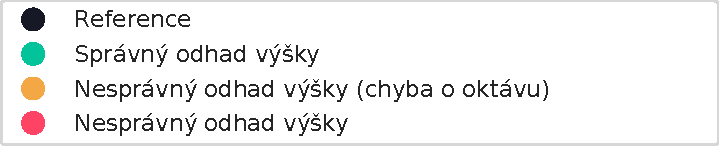
\includegraphics[scale=0.75]{../img/legenda}
\caption{Legenda pro následující kvalitativní srovnání.}
\label{obr:legenda}
\end{figure}

\begin{figure}[h]\centering
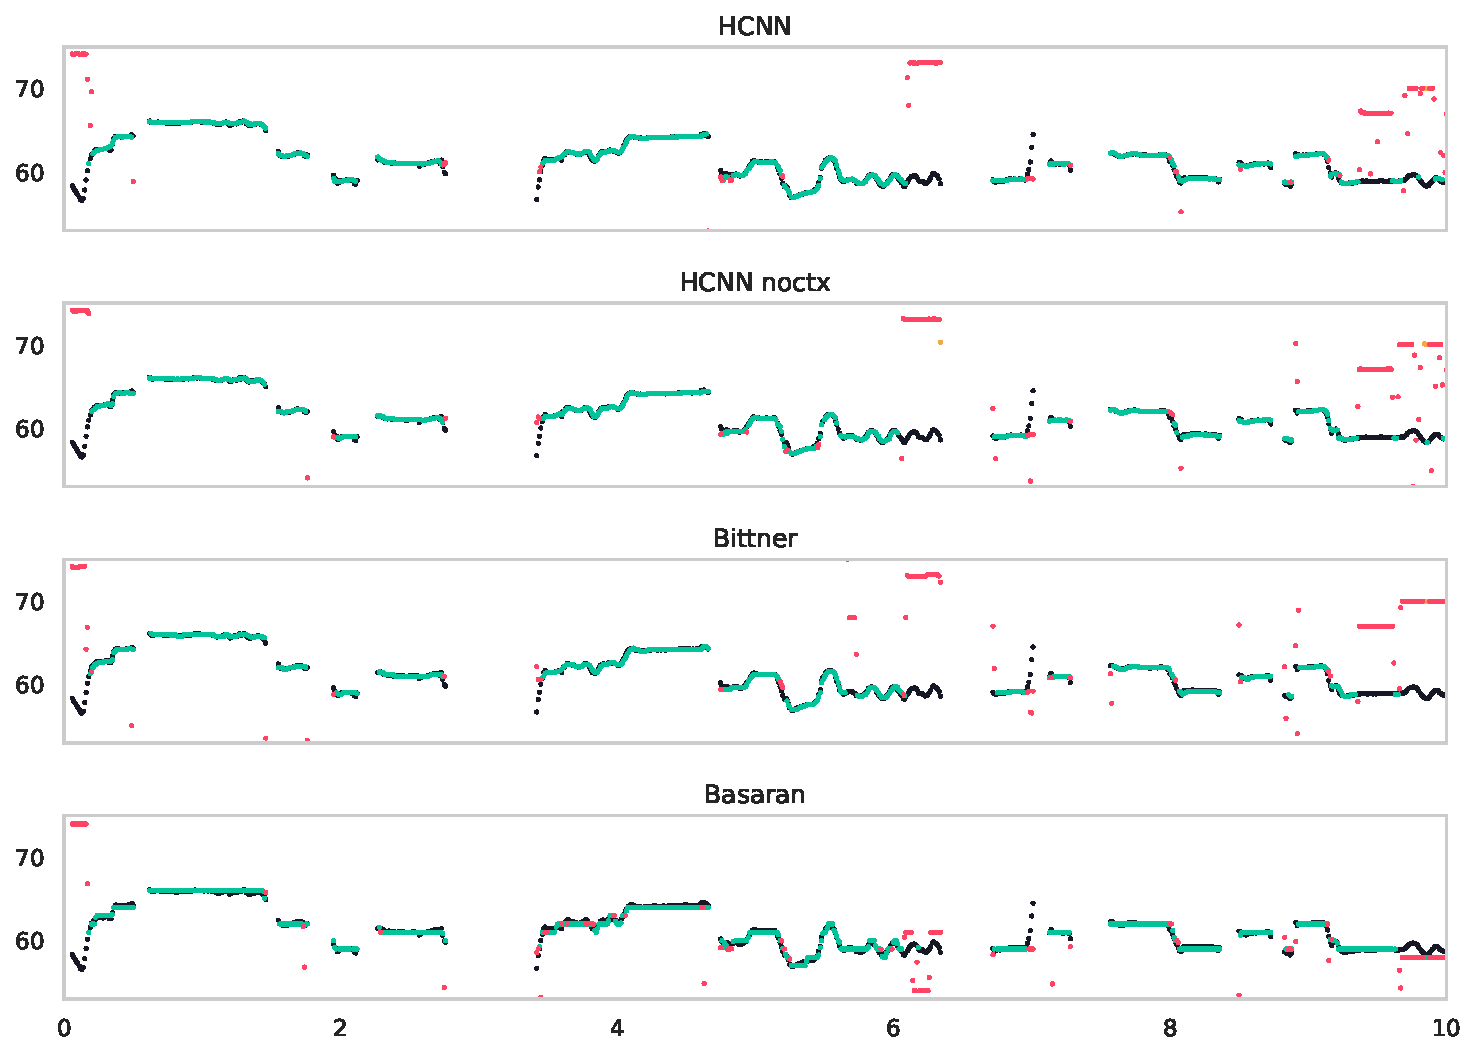
\includegraphics[width=\textwidth,height=\textheight,keepaspectratio]{../img/vysledky/mirex05_train01}
\caption{Příklad s vysokou úspěšností přepisu \texttt{train01} z datasetu MIREX05\-train, se kterým je čtenář seznámen z úvodu práce.}
\label{obr:mirex05_train01}
\end{figure}

Na obrázku \ref{obr:mirex05_train01} můžeme vidět výsledky metod spuštěných na popové nahrávce, ve které melodii nese hlas zpěvačky. Napříč metodami je přepis této nahrávky, kterou uvádíme v úvodu práce, velmi spolehlivý, přesnost odhadu výšky se pohybuje mezi 0.86 a 0.89. Protože v následujících srovnáních ukazujeme zejména chyby přepisu a metody porovnáváme na obtížných příkladech, nechceme, aby si po přečtení sekce čtenář odnesl, že existující metody přepisu nefungují. Proto uvádíme tento příklad (obr. \ref{obr:mirex05_train01}) jako pozitivní ukázku toho, že na obvyklých vstupních datech všechny porovnávané metody fungují velmi dobře.


% \begin{table}[h]
% \centering

%     \begin{tabular}{ll}
%     \toprule
%     Metrika (Metoda) & train10 \\
%     \midrule
%           RPA (HCNN) &   0.917 \\
%           RCA (HCNN) &   0.934 \\
%       RPA (Bittner) &   0.863 \\
%       RCA (Bittner) &   0.868 \\
%       RPA (Basaran) &   0.512 \\
%       RCA (Basaran) &   0.572 \\
%     \bottomrule
%     \end{tabular}

% \caption{Přesnost metod na testovacím souboru \texttt{train10} z datasetu MIREX05.}\label{tab:mirex05_train10}
% \end{table}
\begin{figure}[h]\centering
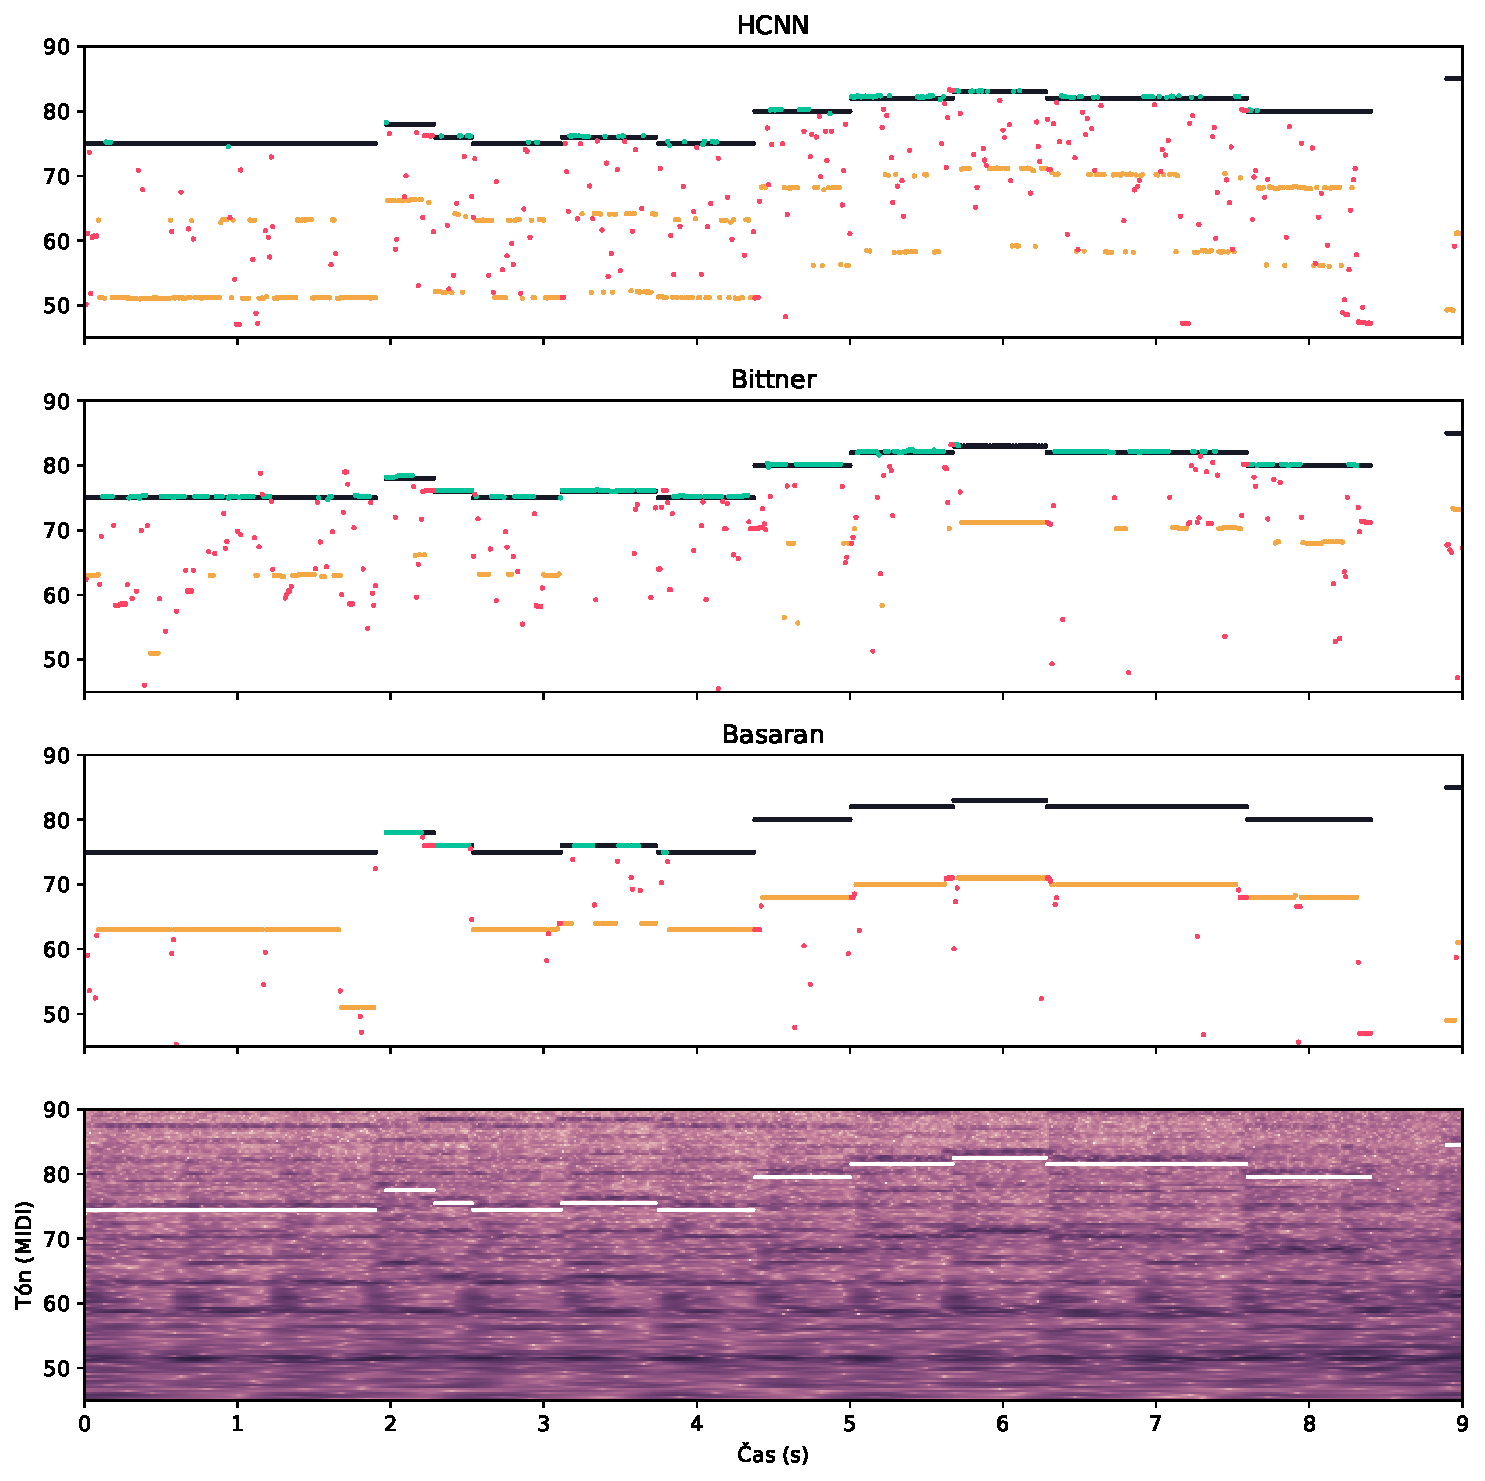
\includegraphics[width=\textwidth,height=\textheight,keepaspectratio]{../img/vysledky/orchset_Musorgski-Ravel-PicturesExhibition-ex6}
\caption{Výstup metod na testovacím souboru \texttt{Musorg\allowbreak{}ski\-Ravel\-Pictures\allowbreak{}Exhibition\-ex6} z datasetu ORCHSET.}
\label{obr:orchset_Musorgski-Ravel-PicturesExhibition-ex6}
\end{figure}

\begin{figure}[h]\centering
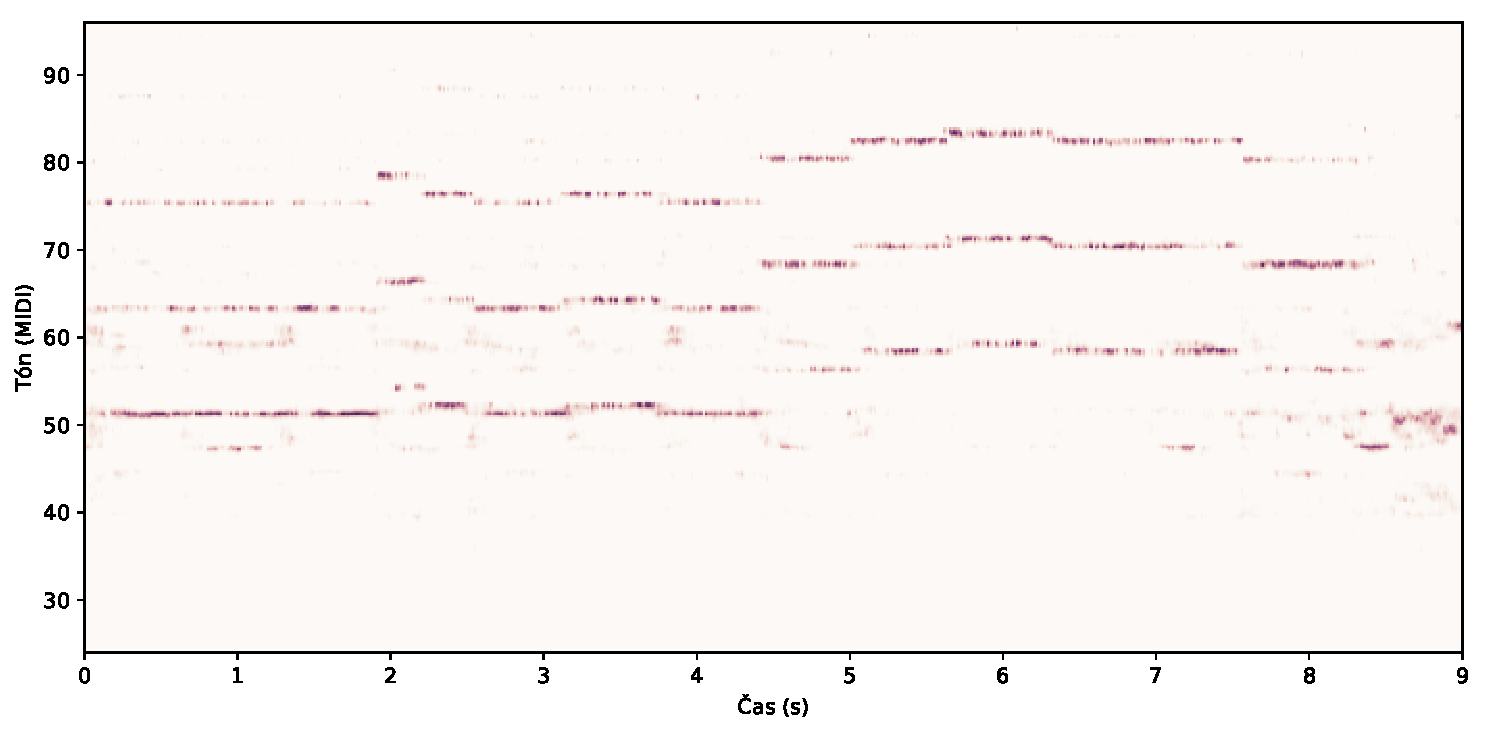
\includegraphics[scale=0.4]{../img/vysledky/orchset_Musorgski-Ravel-PicturesExhibition-ex6_salience}
\caption{Výstupní salience metody HCNN na testovacím souboru \texttt{Musorg\allowbreak{}ski\-Ravel\-Pictures\allowbreak{}Exhibition\-ex6} z datasetu ORCHSET.}
\label{obr:orchset_Musorgski-Ravel-PicturesExhibition-ex6_salience}
\end{figure}

Největší slabinou sítě HCNN noctx se stala podle očekávání časová kontinuita odhadů. Protože tato síť pro odhad výšek uvažuje vždy pouze $5.8\,\rm ms$ vstupu a po vytvoření funkce salience na odhady tónů neaplikujeme žádné způsoby vyhlazování, odhady jednotlivých časových oken na sebe nenavazují. To se nejeví jako zásadní problém v případech, kdy ve skladbě melodii nenese více hlasů v souzvuku (viz výstup \ref{obr:mirex05_train01}, \ref{obr:mirex05_train10}). U některých orchestrálních skladeb však vzniká problém, například pokud melodii nese zároveň sekce smyčců a dechů v různých oktávách. Jak můžeme vidět na výstupu algoritmů \ref{obr:orchset_Musorgski-Ravel-PicturesExhibition-ex6}, HCNN noctx pak \uv{přeskakuje} mezi oktávami. Problém je také dobře vidět na výstupní funkci salience \ref{obr:orchset_Musorgski-Ravel-PicturesExhibition-ex6_salience}, na které vidíme tři totožné kontury posunuté o oktávu. Mírné zlepšení tohoto problému vidíme na výstupech metod HCNN a \cite{Bittner2017}, které sice také nijak výsledek salienční funkce nezpracovávají, na druhou stranu pro její výpočet uvažují delší okna délky $162\,\rm ms$ v případě HCNN a $150\,\rm ms$ v případě metody Bittner. Na obrázku \ref{obr:orchset_Musorgski-Ravel-PicturesExhibition-ex6} vidíme, že množství odhadů těchto metod, je často chybný pouze kvůli nesprávně určené oktávě --- díky většímu kontextu může metoda vybrat v čase navazující odhady a proto tyto výstupy obsahují méně velmi krátkých chybných úseků. Metoda týmu \cite{DBasaranSEssid2018} odhad výšky tónů vyhlazuje pomocí rekurentní architektury GRU, jejich výstup proto obsahuje nejméně skoků, jelikož metoda uvažuje celý kontext skladby, nikoli jen okno omezené délky. Použití rekurentní sítě díky tomu dovoluje zachytit ještě dlouhodobější závislosti a výstupní kontura pak často obsahuje nejmenší množství velmi krátkých, chybných skoků mimo hlavní melodii, které se na obrázku \ref{obr:orchset_Musorgski-Ravel-PicturesExhibition-ex6} hojně vyskytují u metod bez vyhlazování. Na obrázku \ref{obr:orchset_Musorgski-Ravel-PicturesExhibition-ex6} proto vidíme, že metoda \cite{DBasaranSEssid2018} se drží při odhadu jedné oktávy a přesto, že je tato oktáva zvolena špatně, výsledný přepis je koherentní.

% Také je celkový průběh výsledné kontury u této metody častěji . Další výraznou slabinu jsme z analýzy jednotlivých výstupů sítí neregistrovali. U výstupů, ve kterých se sítě nejvíce lišily, byl tento rozdíl nejčastěji způsoben právě těmito diskontinuitami, případně pak zachycením jiného než hlavního nástroje v pozadí. Největší rozdíly ve výsledcích jsou proto na datasetu ORCHSET, ve kterém je výskyt polyfonie nejčastější. 


% \begin{table}[h]
% \centering

%     \begin{tabular}{ll}
%     \toprule
%     Metrika (Metoda) & Musorgski-Ravel-PicturesExhibition-ex6 \\
%     \midrule
%           RPA (HCNN) &                                  0.125 \\
%           RCA (HCNN) &                                  0.725 \\
%       RPA (Bittner) &                                  0.397 \\
%       RCA (Bittner) &                                  0.826 \\
%       RPA (Basaran) &                                  0.040 \\
%       RCA (Basaran) &                                  0.914 \\
%     \bottomrule
%     \end{tabular}

% \caption{Přesnost metod na testovacím souboru \texttt{Musorgski-Ravel-PicturesExhibition-ex6} z datasetu ORCHSET.}\label{tab:orchset_Musorgski-Ravel-PicturesExhibition-ex6}
% \end{table}

\begin{figure}[h]\centering
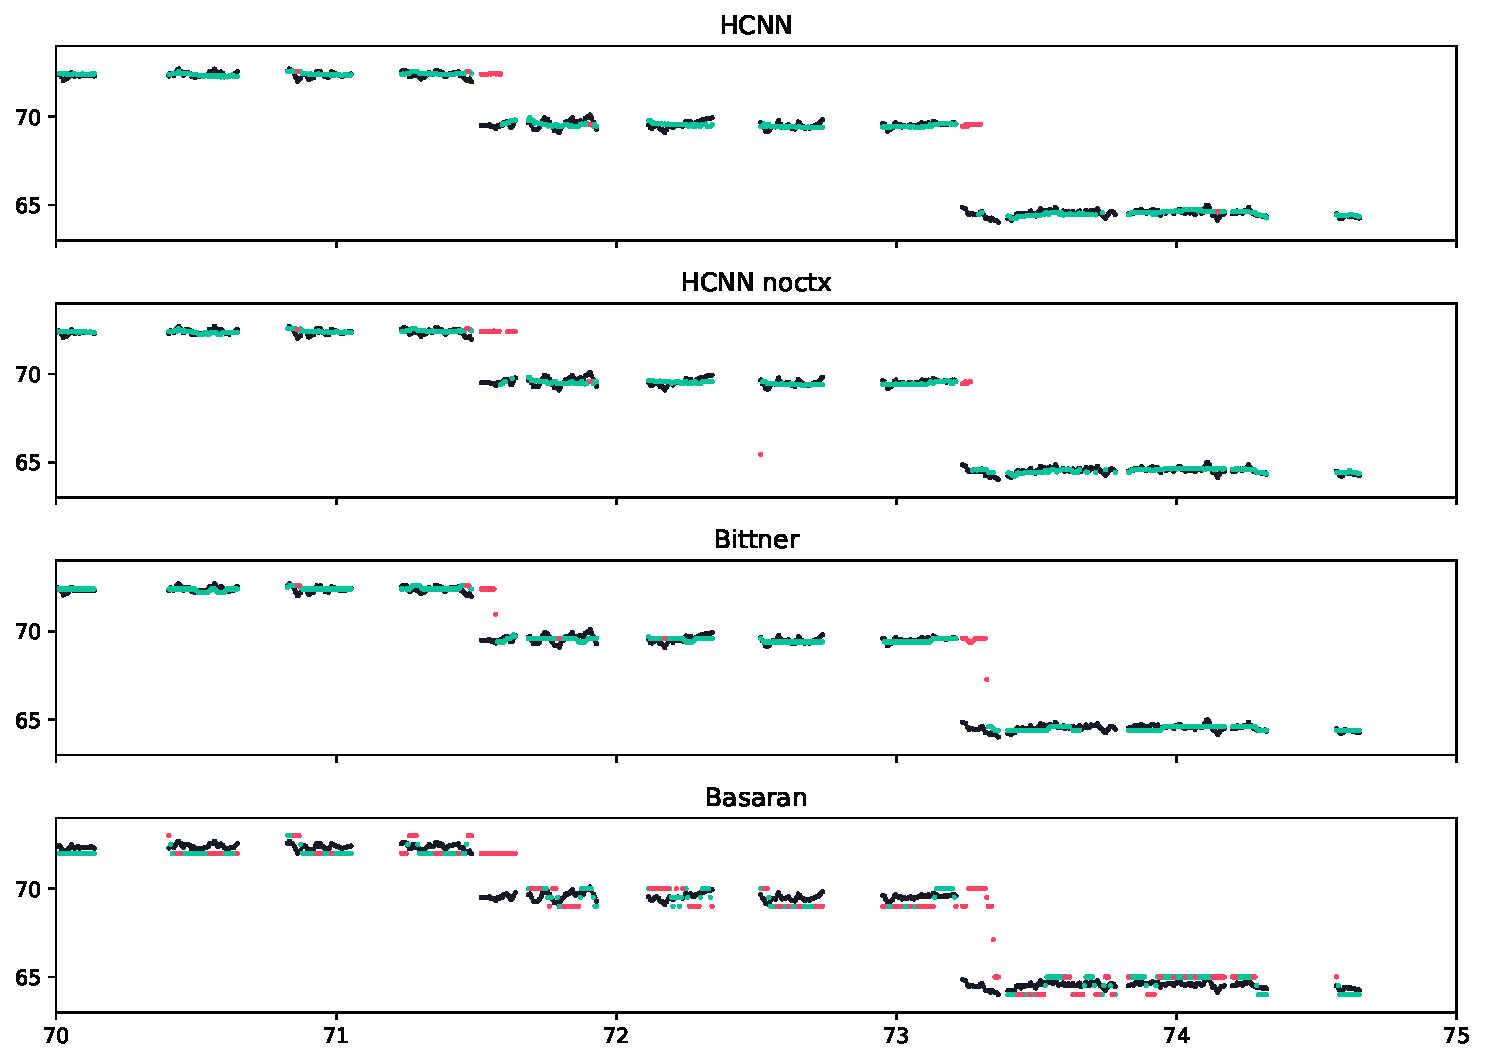
\includegraphics[width=\textwidth,height=\textheight,keepaspectratio]{../img/vysledky/wjazzd_CannonballAdderley_SoWh}
\caption{Detail přepisu metod na testovacím souboru \texttt{Cannonball\allowbreak{}Adderley\allowbreak{}\_\allowbreak{}So\allowbreak{}What} z datasetu WJazzD.}
\label{obr:wjazzd_CannonballAdderley_SoWhat_detail}
\end{figure}


Basaranova metoda pro tuto koherenci výsledných kontur však obětovala frekvenční přesnost znějících výšek tónů, frekvenční rozlišení této metody je totiž na úrovni jednoho půltónu. Jak jsme již prezentovali v kapitole \nameref{cha:experimenty}, výstup metod kvantizovaný na půltóny obsahuje množství chyb navíc, jelikož často selhává v zachycení frekvenčních modulací. Na obrázku \ref{obr:wjazzd_CannonballAdderley_SoWhat_detail} vidíme další limitaci takového výstupu --- pokud je obsah skladby laděný podle jiného referenčního tónu než jaký byl použit pro trénování sítě, znějící tóny vycházejí výškou \uv{mezi} výstupní složky. Z tabulky \ref{tab:wjazzd_CannonballAdderley_SoWhat} je pak zřejmé, že kvůli této kvantizaci síť nedosahuje srovnatelných výsledků, přestože na jiných, žánrově shodných datech, které jsou laděny na správný referenční tón, podává kompetitivní výsledky. Limitace se proto týká zejména jazzových nahrávek pocházejících z období před rokem 1955, před zavedením referenčního tónu A4=440Hz ve standardu ISO16.
\begin{table}[h]
\centering
\begin{tabular}{ll}
\toprule
 Metrika (Metoda) & CannonballAdderley\_SoWhat \\
\midrule
       RPA (HCNN) &                     0.850 \\
 RPA (HCNN noctx) &                     0.848 \\
    RPA (Bittner) &                     0.828 \\
    RPA (Basaran) &                     0.653 \\
\bottomrule
\end{tabular}


% \begin{figure}[h]\centering
% 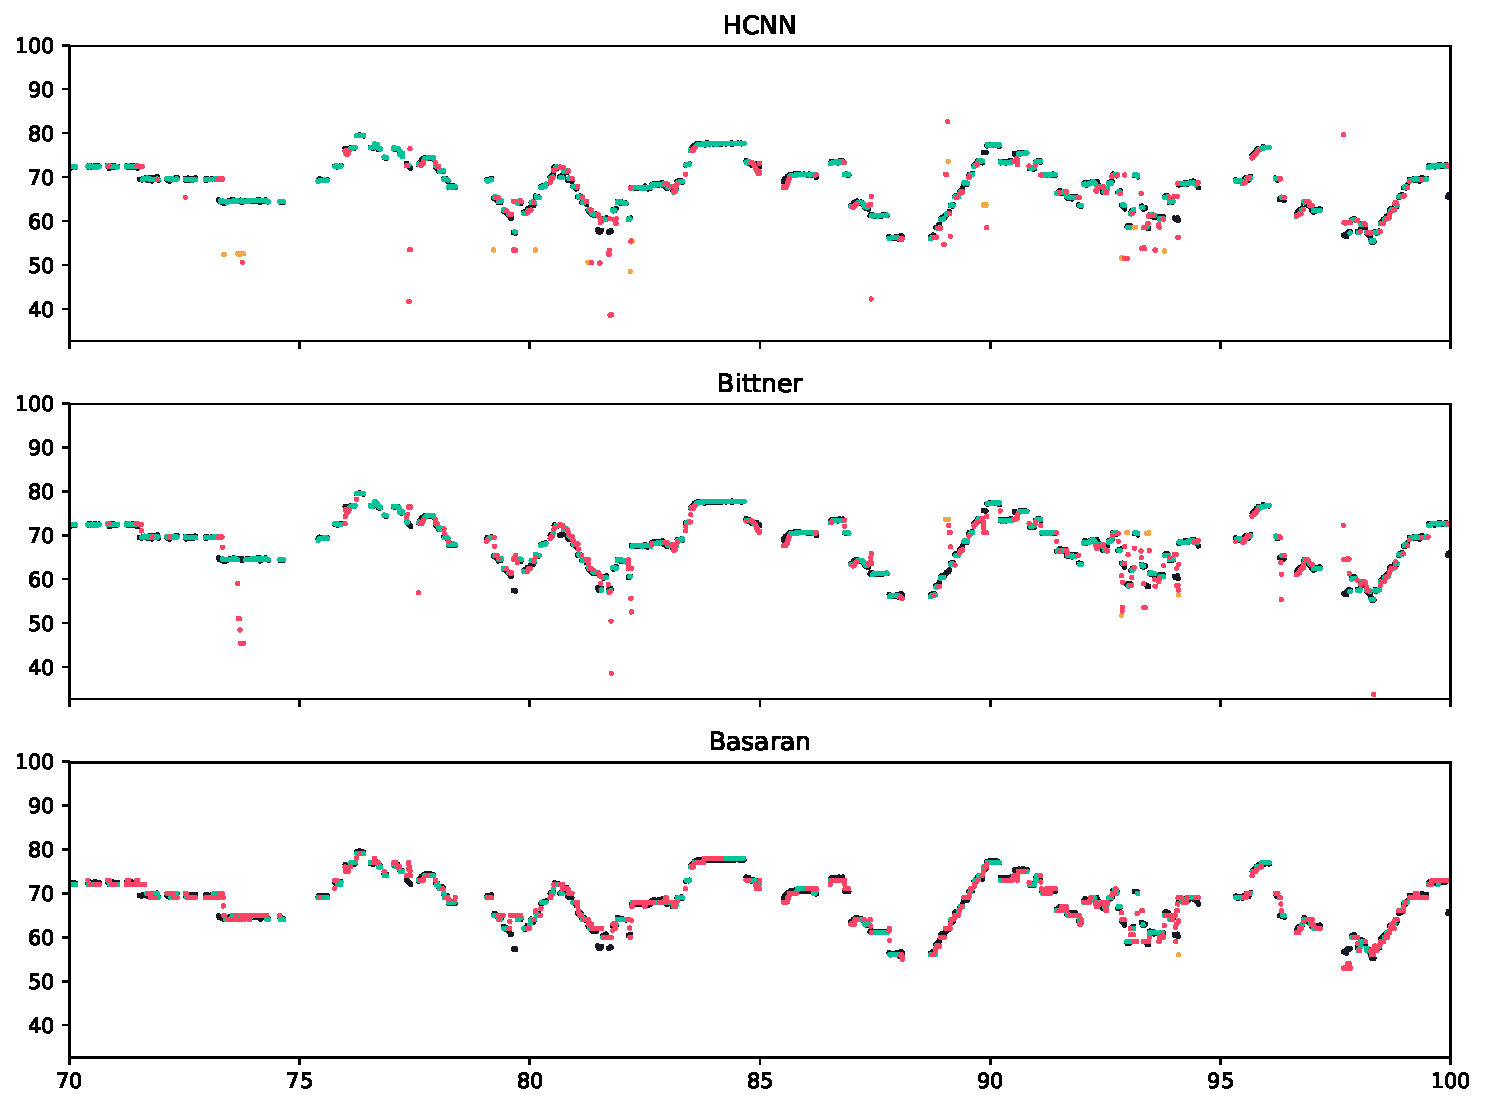
\includegraphics[width=\textwidth,height=\textheight,keepaspectratio]{../img/vysledky/wjazzd_CannonballAdderley_SoWhat}
% \caption{Výstup metod na testovacím souboru \texttt{CannonballAdderley\_SoWhat} z datasetu WJazzD.}
% \label{obr:wjazzd_CannonballAdderley_SoWhat}
% \end{figure}

\caption{Přesnost metod na testovacím souboru \texttt{Cannonball\allowbreak{}Adderley\allowbreak{}\_So\allowbreak{}What} z datasetu WJazzD.}\label{tab:wjazzd_CannonballAdderley_SoWhat}
\end{table}


\begin{figure}[p]\centering
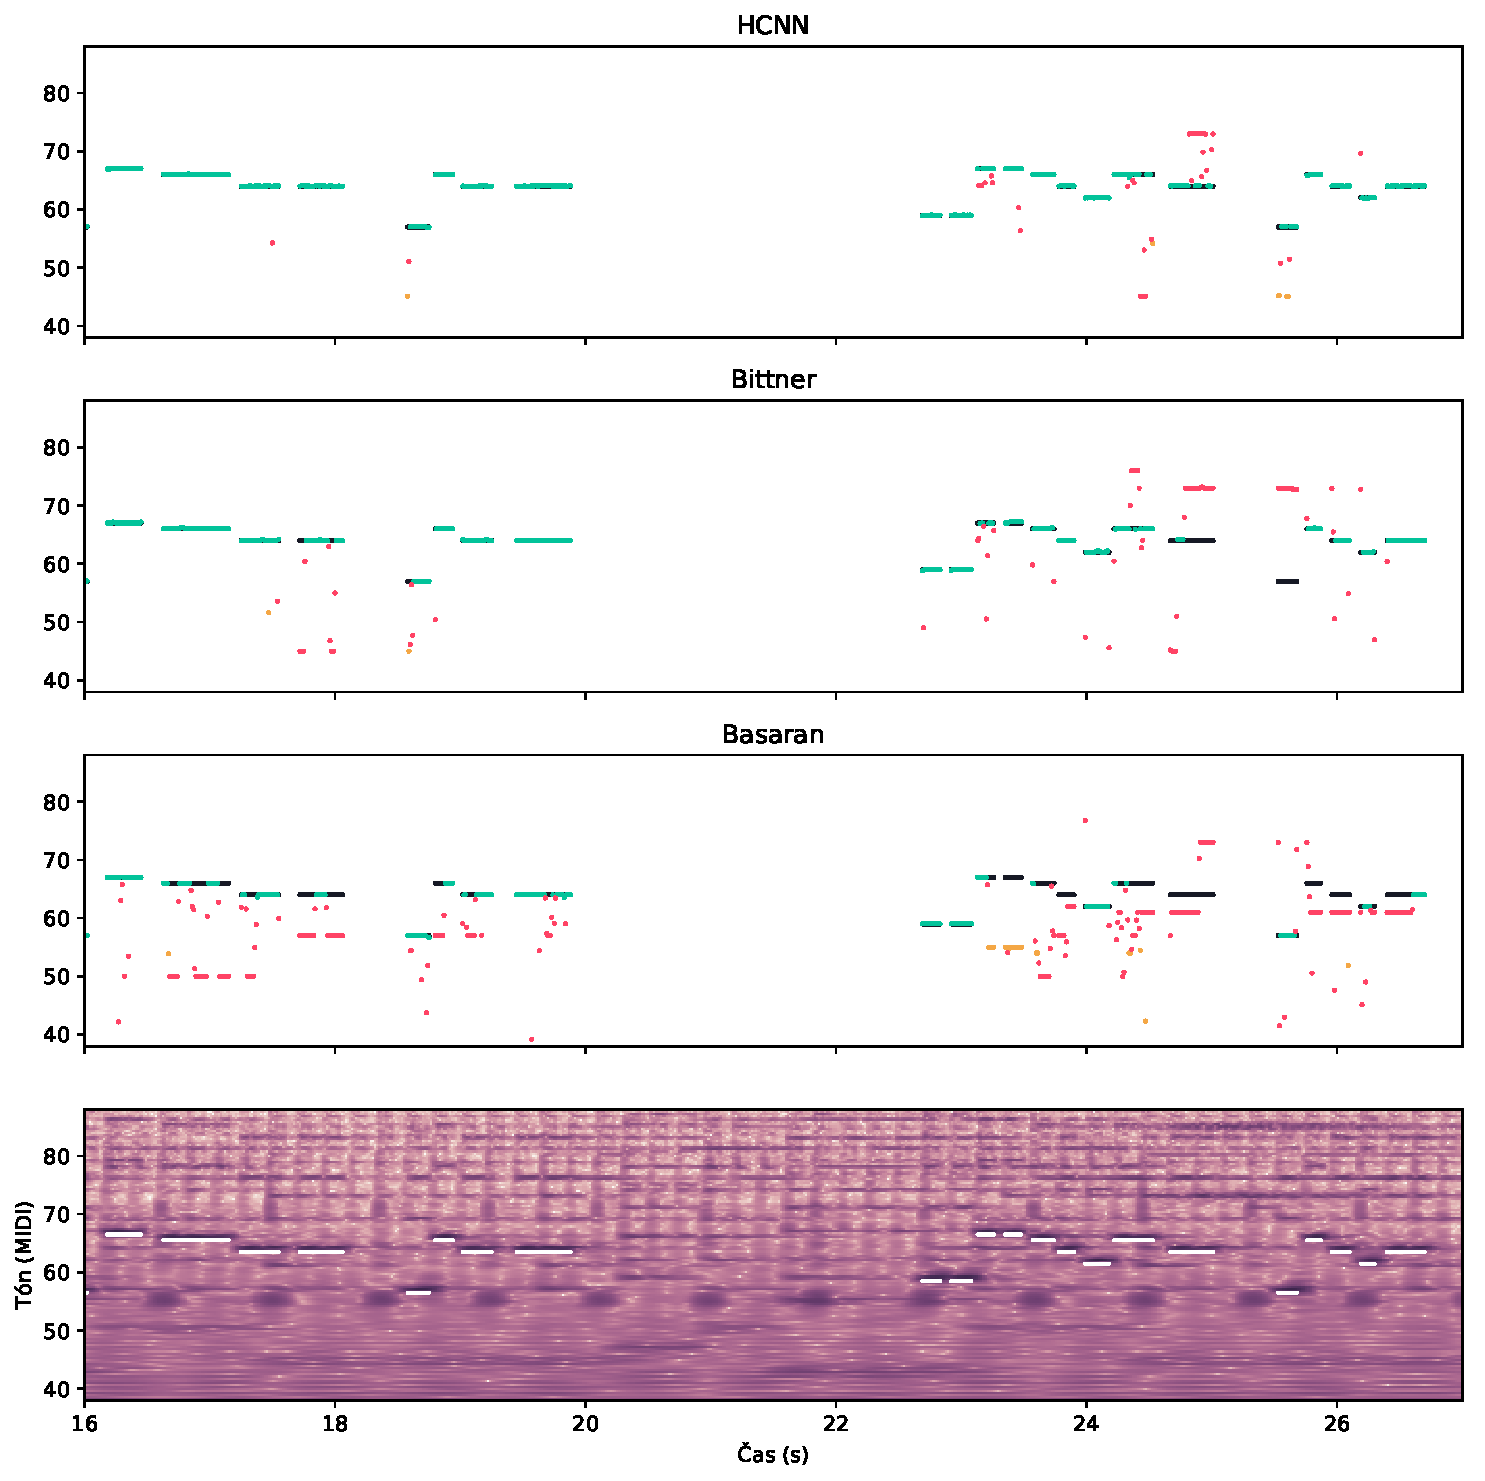
\includegraphics[width=\textwidth,height=\textheight,keepaspectratio]{../img/vysledky/mirex05_train10}
\caption{Výstup metod na testovacím souboru \texttt{train10} z datasetu MIREX05.}
\label{obr:mirex05_train10}
\end{figure}

\begin{figure}[p]\centering
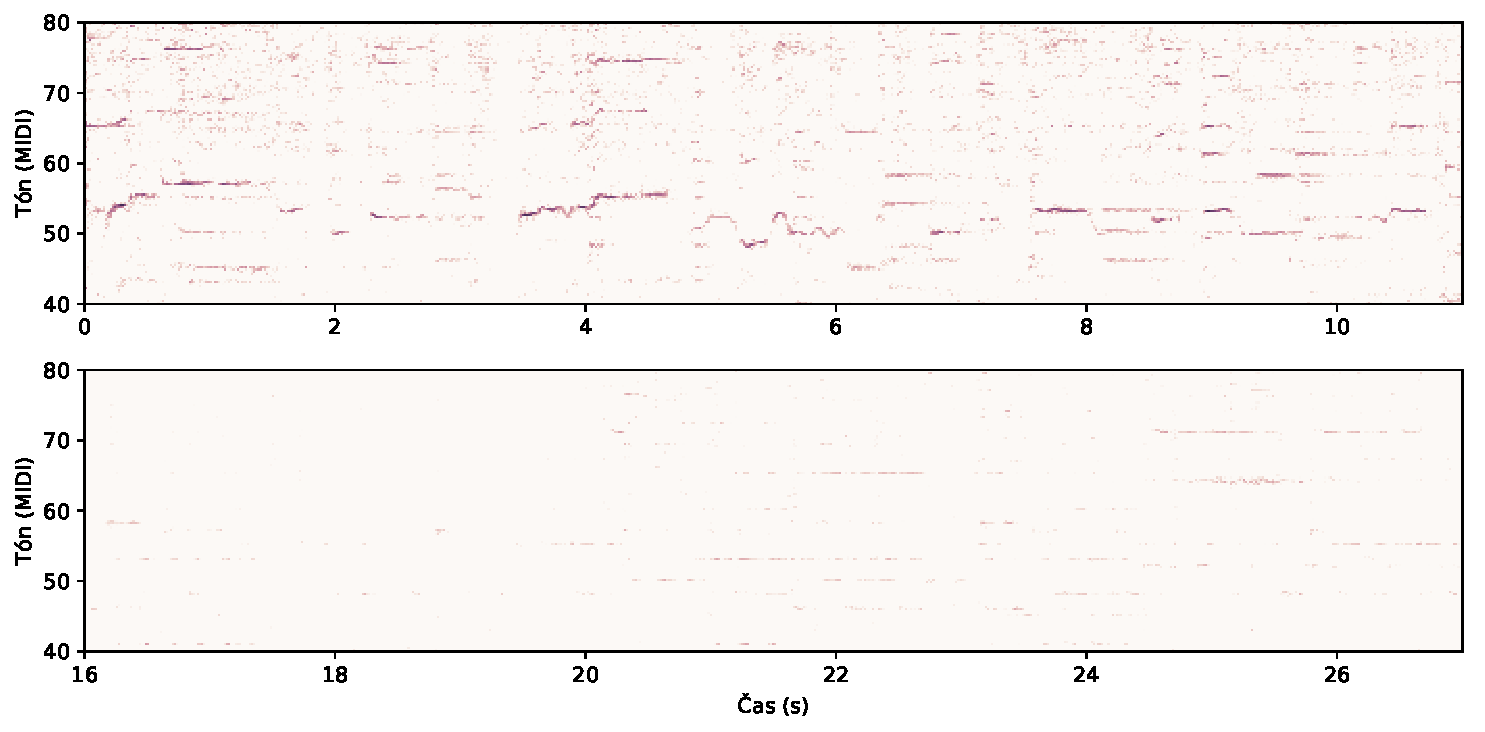
\includegraphics[width=\textwidth,height=\textheight,keepaspectratio]{../img/vysledky/basaran_salience_comparison}
\caption{Srovnání vstupní frekvenčně-časové reprezentace $\bm{\mathrm{H}}^{F_0}$ Basaranovy metody testovacích souborů \texttt{train01} a \texttt{train10} z datasetu MIREX05.}
\label{obr:basaran_salience_comparison}
\end{figure}
Dalším problémem Basaranovy metody je zhoršená schopnost extrakce na syntetických datech. Příklady \texttt{midi2REF}, \texttt{midi3REF}, \texttt{train10REF} z datasetů ADC04 a MIREX05 jsou syntetizovány na základě MIDI pomocí základních zvukových fontů, nahrávky proto zní velmi uměle. Jak vidíme na obrázku \ref{obr:mirex05_train10}, zatímco metody Bittnerové a HCNN si s touto syntetickou barvou hlasu dokáží poradit, výstup Basaranovy metody obsahuje šum a skoky k doprovázejícím nástrojům. Příčinou může být jiná vstupní reprezentace signálu, která je založena na práci \cite{Durrieu2010} a spočívá na modelování hlavního hlasu pomocí zdroje a filtrů. Na obrázku \ref{obr:basaran_salience_comparison} srovnáváme tuto reprezentaci pro vstupní signál s lidským zpěvem (nahoře, \texttt{train01}) a pro signál se syntetickou flétnou (dole, \texttt{train10}). Je zřejmé, že zatímco lidský zpěv tato reprezntace dokáže zachytit, syntetický hlas na reprezentaci téměř zachycen není. 

\begin{figure}[h]\centering
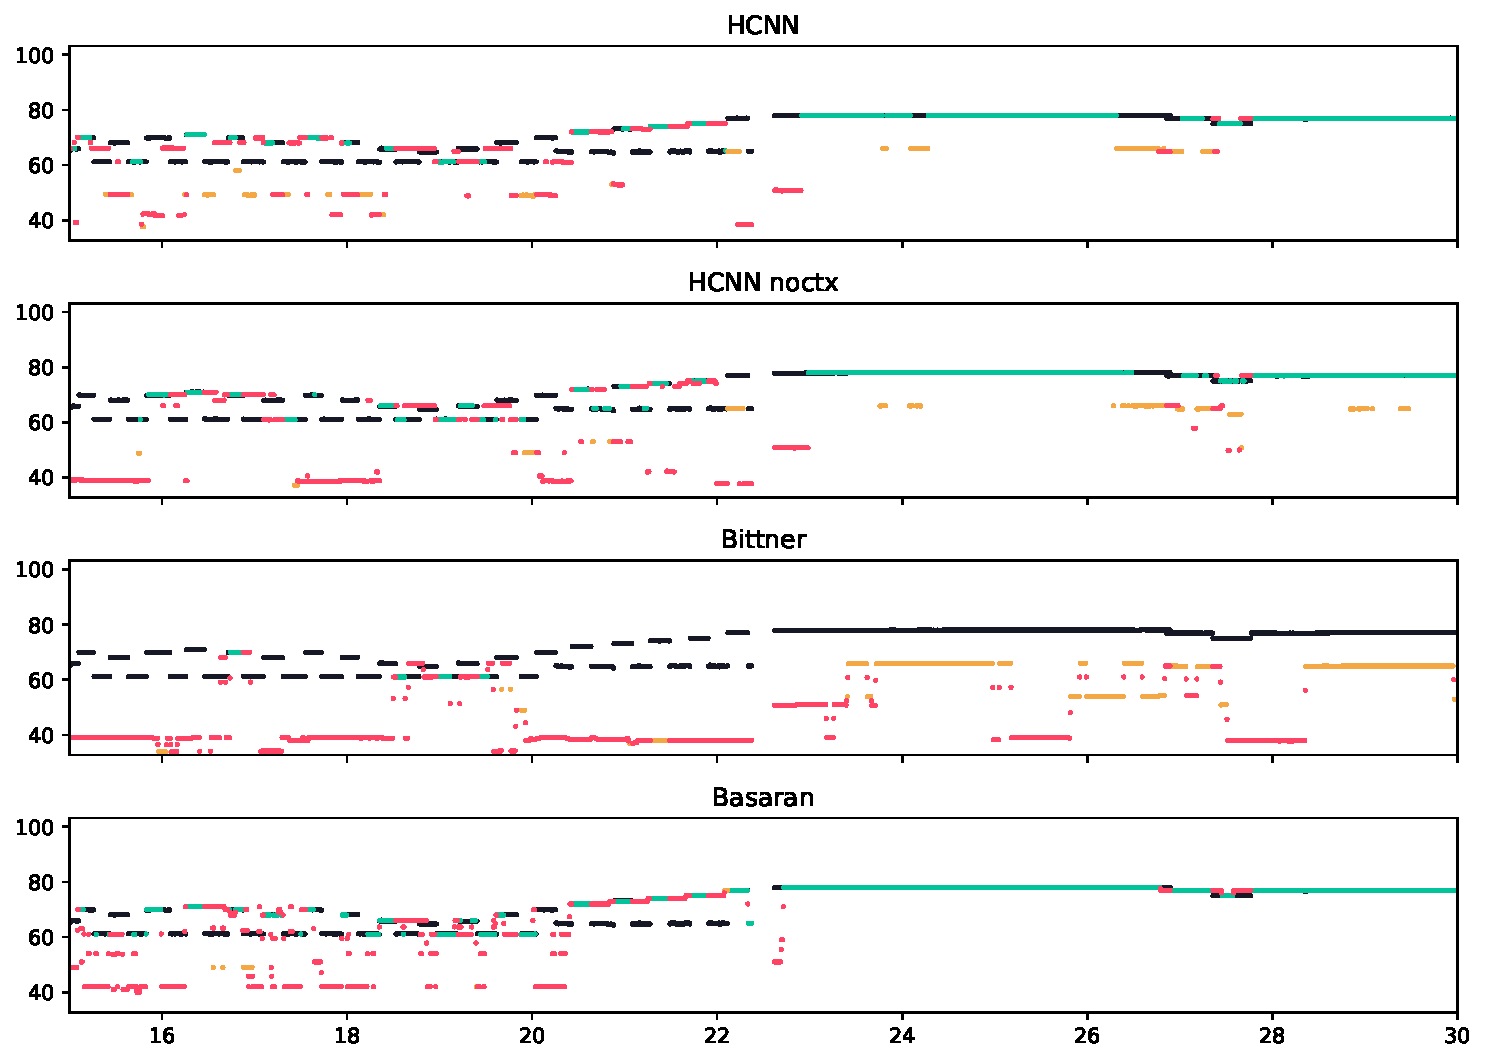
\includegraphics[width=\textwidth,height=\textheight,keepaspectratio]{../img/vysledky/mdb_MatthewEntwistle_FairerHopes}
\caption{Výstup metod na testovacím souboru \texttt{Matthew\allowbreak{}Entwistle\allowbreak{}\_Fairer\allowbreak{}Hopes} z datasetu MedleyDB.}
\label{obr:mdb_MatthewEntwistle_FairerHopes}
\end{figure}
Pokud srovnáme metody HCNN a metodu Bittner, rozdílem v predikcích jsou zejména jiné priority, které přiřazují barvám hlasů. Lze tudíž nalézt mnoho příkladů, kde HCNN zároveň přepisuje melodii a nesprávně místy přeskakuje k nástrojům v doprovodu, zatímco metoda Bittnerové na stejném příkladu tuto chybu nedělá, podobně však existují i opačné příklady. Příkladem, ve kterém se tyto metody nejvíce rozchází, je soubor \texttt{MatthewEntwistle\_FairerHopes} z kolekce MedleyDB, ve kterém melodii hraje harfa. Zvuk harfy se však nevyskytuje v množině trénovacích dat, rozdílem proto je, že zatímco metoda HCNN zvládá alespoň částečně generalizovat i na tuto dosud neslyšenou barvu hlasu, metoda Bittnerové tyto tóny úplně ignoruje a přepisuje doprovod pod harfou (viz obrázek \ref{obr:mdb_MatthewEntwistle_FairerHopes}).

\section{Interpretace výsledků}

Zásadní výhodou metody Basaran oproti HCNN a Bittner je zpracování výsledků funkce salience pomocí rekuretní sítě. Tento rozdíl spolu s jinou výchozí časově-frekvenční reprezentací signálu jeho metodu zvýhodňuje zejména na datasetu ORCHSET, kde jeho metoda v metrice RPA dosahuje o deset procentních bodů lepších výsledků. Pro metodu Basaran je na tomto datasetu také výhodné, že jeho referenční anotace mají půltónové frekvenční rozlišení, tedy stejné, jako výstup této metody. Tudíž jeho metoda při použití tohoto hrubého rozlišení nijak netratí. Na zbylých datasetech se však nižší frekvenční rozlišení projevuje více a metodu pravděpodobně spíše znevýhodňuje. Přesto jsou jeho predikce, zejména pak na složitějších vstupních datech, často koherentnější, obsahují méně šumu. 

Výsledky HCNN a Bittner jsou si oproti výsledkům metody Basaran mnohem podobnější, ačkoliv je mezi nimi větší procentuální rozdíl. Při kvalitativním vyhodnocování jsme nenalezli příliš mnoho příkladů, na kterém by se výstupy metod výrazně lišily. Mezi sítěmi je však řada podobností, zejména stejná vstupní reprezentace, přibližně stejně velký zpracovávaný kontext, přeskočení vyhlazování výstupu ale i celková struktura sítě. Kvantitativní rozdíly na všech datasetech tedy přičítáme spíše lépe naučeným barvám nástrojů a jejich priorit v celkovém mixu. Podobnost výsledků ilustrujeme také výpočtem korelace, zatímco výsledky metriky RPA pro metody Bittner a HCNN mezi sebou mají korelaci 0.932, mezi Basaran a HCNN vychází nižší korelace 0.736.

\section{Online demo}

Pro kvalitativní srovnání výsledků všech metod představovaných v práci je zpřístupněno jednoduché online demo na url \url{http://jirkabalhar.cz:6090/}. 

% \begin{table}[h!]
% \centering

%   \begin{tabular}{ll}
%   \toprule
%   Metrika (Metoda) & MatthewEntwistle\_FairerHopes \\
%   \midrule
%         RPA (HCNN) &                        0.451 \\
%         RCA (HCNN) &                        0.626 \\
%     RPA (Bittner) &                        0.118 \\
%     RCA (Bittner) &                        0.423 \\
%     RPA (Basaran) &                        0.544 \\
%     RCA (Basaran) &                        0.661 \\
%   \bottomrule
%   \end{tabular}

% \caption{Přesnost metod na testovacím souboru \texttt{MatthewEntwistle\_FairerHopes} z datasetu MedleyDB.}\label{tab:mdb_MatthewEntwistle_FairerHopes}
% \end{table}




% \begin{figure}[h]\centering
% 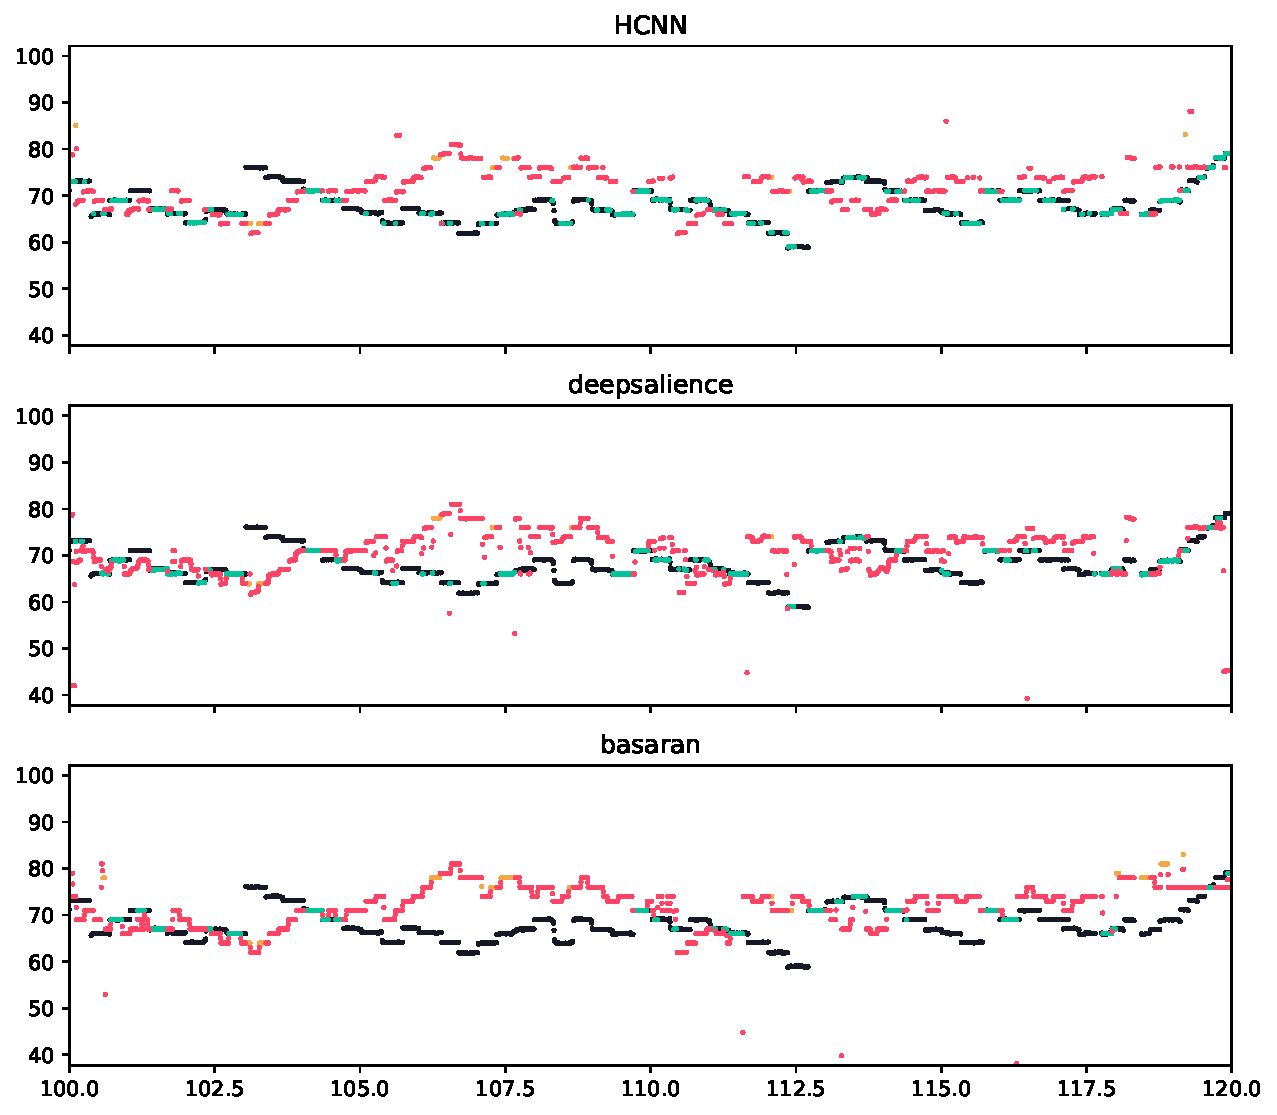
\includegraphics[width=\textwidth,height=\textheight,keepaspectratio]{../img/vysledky/mdb_MusicDelta_Pachelbel}
% \caption{Výstup metod na testovacím souboru \texttt{MusicDelta\_Pachelbel} z datasetu MedleyDB.}
% \label{obr:mdb_MusicDelta_Pachelbel}
% \end{figure}

% \begin{table}[h!]
% \centering

% \begin{tabular}{ll}
% \toprule
% Metrika (Metoda) & MusicDelta\_Pachelbel \\
% \midrule
%       RPA (HCNN) &                0.472 \\
%       RCA (HCNN) &                0.510 \\
%    RPA (Bittner) &                0.461 \\
%    RCA (Bittner) &                0.493 \\
%    RPA (Basaran) &                0.435 \\
%    RCA (Basaran) &                0.491 \\
% \bottomrule
% \end{tabular}

% \caption{Přesnost metod na testovacím souboru \texttt{MusicDelta\_Pachelbel} z datasetu MedleyDB.}\label{tab:mdb_MusicDelta_Pachelbel}
% \end{table}

